\section{Gateway}
Per unificare le chiamate da e verso l'esterno su un'unica porta, si è deciso di implementare un gateway.
Questo può comportare significativi vantaggi anche per sviluppi futuri:
\begin{itemize}
    \item Può agire come un punto di ingresso sicuro per l’applicazione, filtrando e autenticando le richieste provenienti dall’esterno;
    \item Permette meccanismi di caching; 
\end{itemize}

Permette inoltre di astrarre la composizione interna del servizio dal punto di vista del client, il quale vedrà il sistema come un unica entità con un unico punto d'accesso.

\subsection{Component Diagram}
A seguito dell'aggiunta di questo microservizio, viene quindi aggiornato il diagramma dei componenti.

\begin{figure}[htbp]
	\centering
	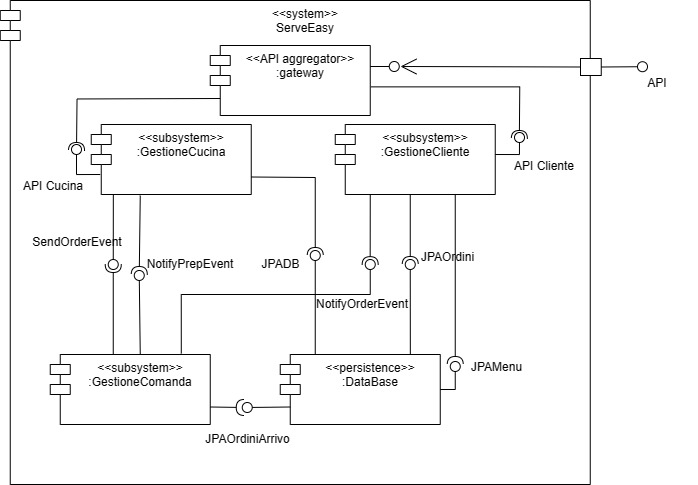
\includegraphics[scale=0.35]{iterazione3/images/component_gateway.jpg}
	\caption{Component Diagram con Gateway
 \label{fig:componentgateway}}
\end{figure}

\subsection{Deployment Diagram}
Viene aggiunto un nodo alla rete di container, il quale è l'unico ad esporre un'interfaccia all'esterno.



\begin{figure}[htbp]
	\centering
	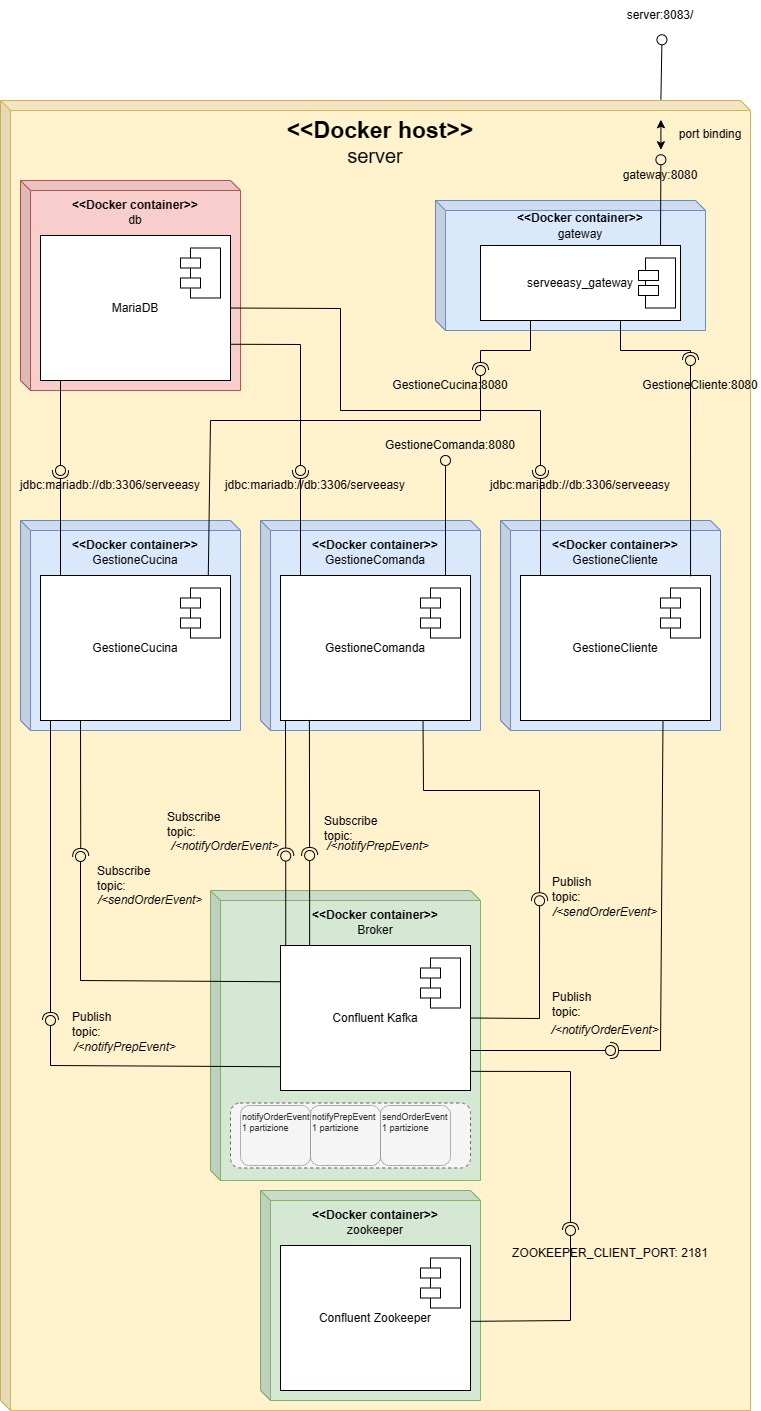
\includegraphics[scale=0.35]{iterazione3/images/Deployment_iterazione3.jpg}
	\caption{Deployment Diagram con gateway
 \label{fig:deploymentdiagram}}
\end{figure}
\clearpage